% See exam.cls and examdoc.tex for the license information
\documentclass[12pt, answers]{exam}

\usepackage{amssymb}
\usepackage{makeidx}
\usepackage{amsmath}
\usepackage{graphicx}
\usepackage{caption}
\usepackage{tabulary}
\usepackage{color}
\usepackage{multicol}
\usepackage{multirow}
\usepackage{enumerate}
\usepackage{float}
\usepackage{colortbl}
\usepackage[table,xcdraw]{xcolor}
\usepackage{array}

\newcolumntype{C}[1]{>{\centering\let\newline\\\arraybackslash\hspace{0pt}}m{#1}}

\addpoints

% In case we're not using hyperref.sty:
\providecommand{\texorpdfstring}[2]{#1}
% The following can be used in \section commands
% without generating pdf warnings:
\newcommand{\bs}{\texorpdfstring{\char`\\}{}}

\makeindex

\newcommand{\indc}[1]{\index{#1@\texttt{\char`\\#1}}}
\newcommand{\indcsub}[2]{\index{#1@\texttt{\char`\\#1}!#2}}
\newcommand{\indcstart}[1]{\index{#1@\texttt{\char`\\#1}|(}}
\newcommand{\indcstop}[1]{\index{#1@\texttt{\char`\\#1}|)}}

\newcommand{\indt}[1]{\index{#1@\texttt{#1}}}
\newcommand{\indtsub}[2]{\index{#1@\texttt{#1}!#2}}
\newcommand{\indtstart}[1]{\index{#1@\texttt{#1}|(}}
\newcommand{\indtstop}[1]{\index{#1@\texttt{#1}|)}}

\extraheadheight{-.4in}

\pagestyle{headandfoot}
%\extraheadheight{.2 in}
\firstpageheader{}{}{}
\runningheader{}{}{}
\firstpagefooter{}{Construction of scoring matrix}{Page \thepage\ of \numpages}
\firstpagefootrule
\runningfooter{}{Construction of scoring matrix}{Page \thepage\ of \numpages}
\runningfootrule

%---------------------------------------------------------------------

\shadedsolutions
\noprintanswers
\definecolor{SolutionColor}{rgb}{0.8,0.9,1}

\setcounter{section}{10}

\begin{document}

\section{Exercises -- Construction of scoring matrix}

%---------------------------------------------------------------------
\begin{questions}

%%% Question 1
\question \textbf{Scoring schemes for protein alignments}

Calculate the score of the alignment by using different scoring schemes.

\begin{verbatim}
    Seq1 R-HIC
    Seq2 RDDCC
\end{verbatim}

\begin{parts}

\vspace{0.1 in}

%% (a)
  \part Use the identity with a simple scoring scheme as match: 1, mismatch: 0, and gap penalty: 0.

\begin{solution}[0.35 in]
2
\end{solution}

%% (b)
  \part Use the genetic code.

\begin{table}[h]
\footnotesize
\begin{center}
\begin{tabular}{|c|cccc|c|}
\hline
\itshape First  & \multicolumn{4}{c|}{\itshape Second position} & \itshape Third \\
\cline{2-5}
\itshape position & \makebox[2em]{T} & \makebox[2em]{C} & \makebox[2em]{A} & \makebox[2em]{G} & \itshape position \\ 
\hline
   & F & S & Y & C & T \\
   & F & S & Y & C & C \\
\raisebox{1.5ex}[0mm]{T} & L & S & \itshape Stop & \itshape Stop & A \\
   & L & S & \itshape Stop & W & G \\ 
\hline
   & L & P & H & R & T \\
   & L & P & H & R & C \\
\raisebox{1.5ex}[0mm]{C}    & L & P & Q & R & A \\
   & L & P & Q & R & G \\ 
\hline
   & I & T & N & S & T \\
   & I & T & N & S & C \\
\raisebox{1.5ex}[0mm]{A}    & I & T & K & R & A \\
   & M & T & K & R & G \\ 
\hline
   & V & A & D & G & T \\
   & V & A & D & G & C \\
\raisebox{1.5ex}[0mm]{G}    & V & A & E & G & A \\
   & V & A & E & G & G \\ 
\hline
\end{tabular}
%\epsfig{file=gencode.eps,width=.25\textwidth}
\qquad
\begin{tabular}{lll}
A & Ala & Alanine \\
C & Cys & Cysteine \\
D & Asp & Aspartic acid \\
E & Glu & Glutamic acid \\
F & Phe & Phenylalanine \\
G & Gly & Glycine \\
H & His & Histidine \\
I & Ile & Isoleucine \\
K & Lys & Lysine \\
L & Leu & Leucine \\
M & Met & Methionine \\
N & Asn & Asparagine \\
P & Pro & Proline \\
Q & Gln & Glutamine \\
R & Arg & Arginine \\
S & Ser & Serine \\
T & Thr & Threonine \\
V & Val & Valine \\
W & Trp & Tryptophan \\
Y & Tyr & Tyrosine
\end{tabular}
\end{center}
\end{table}

\begin{solution}[1 in]
9
\begin{verbatim}
         CGU --- CAU AUU UGU
         CGU GAU GAU UGU UGU
\end{verbatim}
\end{solution}

%% (c)
  \part Use the AACH.

\begin{figure}[H]
      \centering
      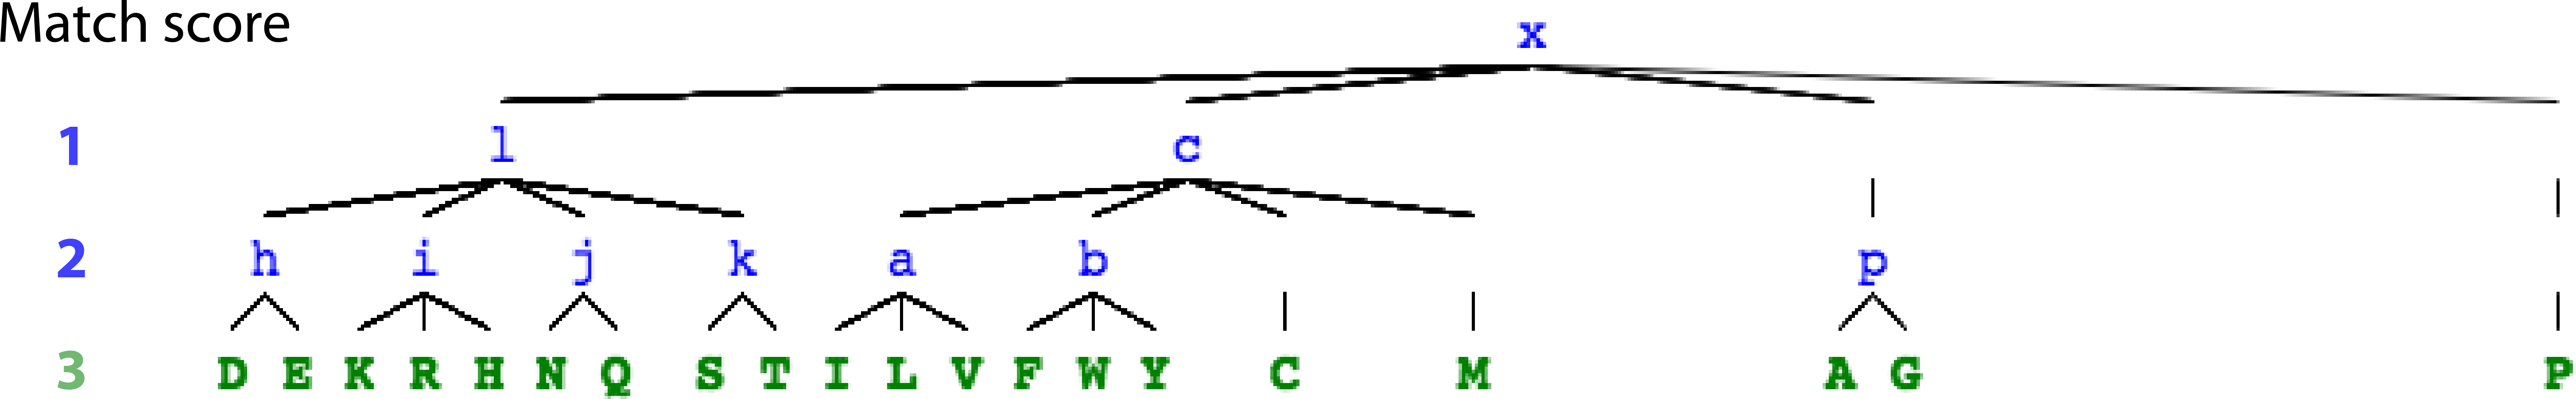
\includegraphics[width=0.7 \textwidth]{fig11/aach.png}
\end{figure}

\begin{solution}[0.35 in]
3 + 0 + 1 + 1 + 3 = 8
\end{solution}

\end{parts}


\newpage

%%% Question 2
\question \textbf{Probabilities of accepted mutations}

Use a phylogenetic tree below to calculate the probabilities of accepted mutations. The tree contains sequences of four OTUs.

\begin{figure}[H]
      \centering
      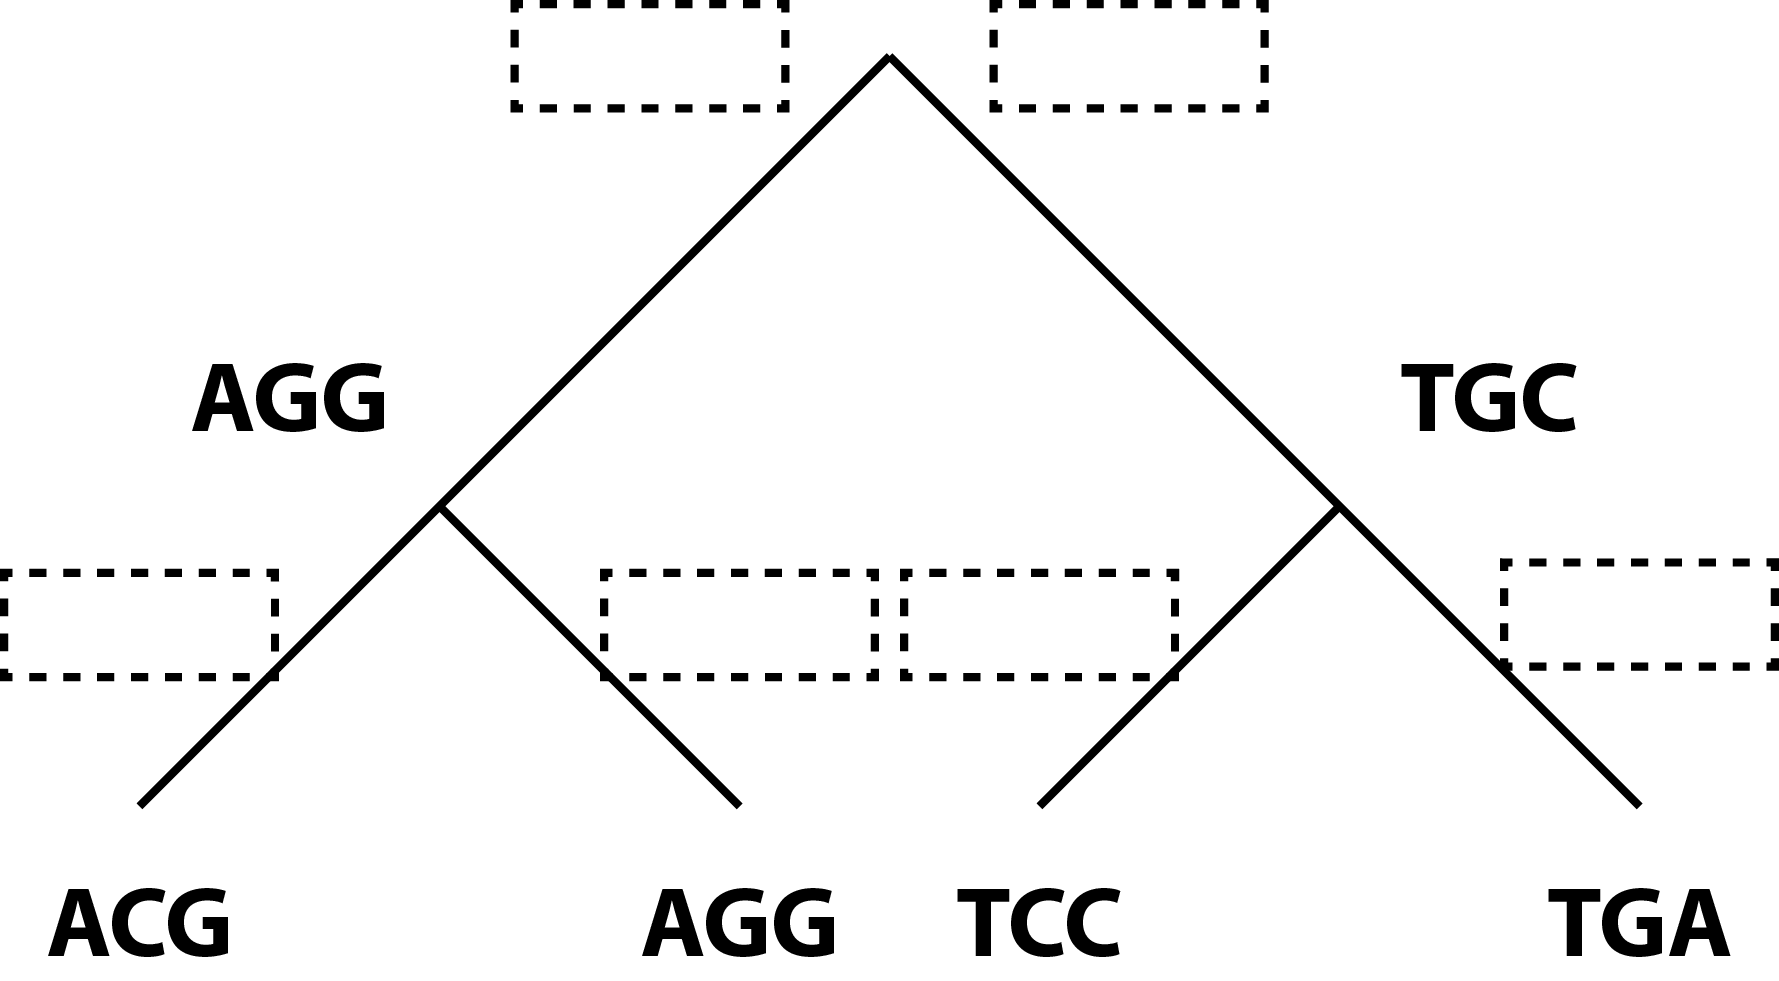
\includegraphics[width=0.4 \textwidth]{fig11/tree.png}
\end{figure}

\begin{parts}

\vspace{0.1 in}

%% (a)
  \part Estimate the mutations and fill them in the boxes next to the edges.
  
  \bigskip 

%% (b)
  \part Count the occurrences of mutations and fill them in the matrix. Note that a mutation A $\rightarrow$ B is equivalent with a mutation B $\rightarrow$ A.

\begin{table}[H]
\centering
\begin{tabular}{|c|c|c|c|c|}
\hline
  & A & C & G & T \\ \hline
A &   &   &   &   \\ \hline
C &   &   &   &   \\ \hline
G &   &   &   &   \\ \hline
T &   &   &   &   \\ \hline
\end{tabular}
\end{table}

%% (c)
  \part Use the following definitions and calculate $f_{CG}$, $f_C$ and $f$.
\begin{align*}
f_{ab} &: \text{The number of mutations from } a \text{ to } b \text{ or from } b\text{ to } a \\
f_a &: \text{Total number of mutations in which } a \text{ takes part} \\
f &: \text{Twice the total number of mutations} \\ \\
f_{CG} &: \\
f_C &: \\
f &:  \\
\end{align*}

%% (d)
  \part 	Use the following definition and calculate $p_C$.
\begin{align*}
p_a &: \text{The relative occurrence of } a \text{ in the observed sequences} \\ \\
p_C &:  
\end{align*}

\end{parts}


\newpage

%%% Question 3
\question \textbf{Relative mutability of PAM}

Relative mutability is calculated from frequencies of estimated mutilation and background probabilities.

\begin{align*}
m_a &:  \dfrac{1}{100p_a}  \times \dfrac{f_a}{f} \\ \\
f_a &:  \text{The total number of point mutations in which } a \text{ takes part}  \\
f &:  \text{Twice the total number of point mutations} \\ \\
p_a &: \text{The relative occurrence of } a \text{ in the observed sequences}
\end{align*}

\noindent
Assume that the frequencies are pre-calculated as follows.
\begin{itemize}
\item Frequencies of estimated mutations \\ \\
 $f_A: 2, \quad f_G: 3, \quad f_C: 3, \quad f_T: 2$ \\
 $f: 10$ \\

\item Background probabilities \\ \\
 $p_A: 3/10, \quad p_G: 2/10, \quad p_C: 4/10, \quad p_T: 1/10 $
 
\end{itemize}

\begin{parts}

\vspace{0.1 in}

%% (a)
  \part Calculate the probabilities of point mutations by $\dfrac{f_a}{f}$. \\
  
 $\dfrac{f_A}{f}:
 \quad  \quad \quad
 \dfrac{f_G}{f}:
 \quad \quad  \quad
 \dfrac{f_C}{f}:
 \quad \quad  \quad
 \dfrac{f_T}{f}: $ \\

%% (b)
  \part 	Calculate $100p_a$. \\

 $100p_A:
 \quad  \quad \quad
 100p_G:
 \quad  \quad \quad
 100p_C:
 \quad  \quad \quad
 100p_T: $ \\

%% (c)
  \part Calculate the relative mutability $m_a$. \\

 $m_A: 
 \quad  \quad \quad
 m_G: 
 \quad  \quad \quad
 m_C:
 \quad \quad \quad
  m_T:  $ \\

\end{parts}


\newpage

%%% Question 4
\question \textbf{Mutation probabilities of PAM}

Mutation probabilities are calculated from relative mutability.
\begin{align*}
m_{ab} &: m_a \times \dfrac{f_{ab}}{f_a},  \quad \quad  m_{aa} : 1 - m_a \\
f_{ab} &:  \text{Total number of point mutations in which } a \text{ takes part}  \\
f_a &:  \text{Twice the total number of point mutations} \\ 
m_a &: \text{Relative mutability of } a 
\end{align*}

\noindent
Assume that the frequencies are pre-calculated as follows.
\begin{itemize}
\item Frequencies of estimated mutations \\ \\
 $f_{AC}: 8, \quad f_A: 32$ \\

\item Relative mutability \\ \\
 $m_A: 0.004 $
 
\end{itemize}

\begin{parts}

\vspace{0.1 in}

%% (a)
  \part 	Calculate $M_{AC}$. 
  
\begin{solution}[0.35 in]
$0.004 \times \frac{8}{32} = 0.001$
\end{solution}

%% (b)
  \part Calculate $M_{AA}$.

\begin{solution}[0.35 in]
$1 - 0.004 = 0.996$
\end{solution}

\end{parts}


\bigskip 

%%% Question 5
\question \textbf{Odds ratios of PAM}

Odds ratios are calculated from mutation probabilities and background probabilities.
\[
O_{ab} = \dfrac{M_{ab}}{p_b} 
= m_a \times \dfrac{f_{ab}}{f_a} \times \dfrac{1}{f_b}
= \dfrac{1}{100} \times \dfrac{f_{ab}}{f} \times \dfrac{1}{p_{a}p_{b}}
\]

\noindent
Assume that the frequencies are pre-calculated as follows.
\begin{center}
$f_{AC}: 16, \quad f: 400, \quad p_A: 0.2, \quad p_c: 0.4 $
\end{center}

\begin{parts}

\vspace{0.1 in}

%% (a)
  \part Calculate $O_{AC}$.
  
\begin{solution}[0.35 in]
$(1/100) \times (16/400) \times (1/(0.2 \times 0.4)) = 0.005$
\end{solution}

%% (b)
  \part Calculate $O_{CA}$.

\begin{solution}[0.35 in]
$0.005$
\end{solution}

\end{parts}



%%% Question 6
\question \textbf{BLOSUM}

BLOSUM uses several thousand blocks to calculate the probabilities of accepted mutation. Use the following definitions and Block1 \& Block2 to solve the problems.
\begin{align*}
f_{ab}:& \text{ Frequencies of an observed pair } a \text{ and } b. \\
T:& \text{ Total number of pairs from all blocks. } \\
 & \text{ The number of pairs can be calculated as } 1/2wm(m-1). \\
p_a:& \text{ } p_a = f_{aa} + \sum_{e \neq a} f_{ae}/2 \\
e_{aa}:&  \text{ } p_a p_a \\
e_{ab}:&  \text{ } p_a p_b + p_b p_a = 2 p_a p_b
\end{align*}
\begin{table}[H]
\centering
\begin{tabular}{ll}
Block1 & Block2 \\
CAGC   & GGA    \\
GTAC   & GTA    \\
CAGC   &       
\end{tabular}
\end{table}

\begin{parts}

%% (a)
  \part Count the occurrences of all pairs.
  
\begin{table}[H]
\centering
\begin{tabular}{|c|c|c|c|c|}
\hline
  & A & C & G & T \\ \hline
A &   &   &   &   \\ \hline
C &   &   &   &   \\ \hline
G &   &   &   &   \\ \hline
T &   &   &   &   \\ \hline
\end{tabular}
\end{table}

%% (b) 
  \part Calculate $T$.

\begin{solution}[0.35 in]
$(1/2 \times 4 \times 3 \times 2) + (1/2 \times 3 \times 2 \times 1) = 12 + 3 = 15$
\end{solution}  
 
%% (c) 
  \part Calculate $f_{AA}$ and $f_{AG}$.

\begin{solution}[0.35 in]
$f_{AA} : 2/15, \quad  f_{AG} : 2/15$
\end{solution}  

%% (d) 
  \part Calculate $p_A$ and $p_G$.

\begin{solution}[0.35 in]
$p_A : 8/30, \quad  p_G : 9/30$
\end{solution}  

%% (e) 
  \part Calculate $e_{AA}$ and $e_{AG}$.

\begin{solution}[0.35 in]
$e_{AA} : 64/900, \quad  e_{AG} : 144/900$
\end{solution}  

%% (f) 
  \part Calculate $f_{AA}/e_{AA}$ and $f_{AG}/e_{AG}$.

\begin{solution}[0.35 in]
$f_{AA}/e_{AA} : 1.875, \quad  f_{AG}/e_{AG} : 0.833$
\end{solution}  

\end{parts}


\end{questions}
%---------------------------------------------------------------------
       
\end{document}

